\documentclass[]{article}
\usepackage{caption,subcaption,graphicx,float,url,amsmath,amssymb,amsthm,tocloft,cancel,thmtools,gensymb,braket,bm}
\usepackage[toc,nonumberlist]{glossaries}
\usepackage{glossaries-extra}
\usepackage[toc,page]{appendix}

\newcommand\numberthis{\addtocounter{equation}{1}\tag{\theequation}}

\newtheorem{thm}{Theorem}
\newtheorem{defn}[thm]{Definition}
\newtheorem{cor}[thm]{Corollary}
\newtheorem{lemma}[thm]{Lemma}
\graphicspath{{figs/}}
\widowpenalty10000
\clubpenalty10000
\setcounter{tocdepth}{2}

%opening
\title{Theoretical Minimum\\Particle Physics 2\\Standard Model}
\author{Simon Crase(compiler)}

\begin{document}

\maketitle

\begin{abstract}
These are my notes for the \emph{New Revolutions in Particle Physics 2} lectures from Leonard Susskind's \emph{Theoretical Minimum} series\cite{susskind2009standard}. Since this material predates the discovery of the Higgs Boson, there is an appendix \emph{Demystifying the Higgs Boson} \cite{susskind2010demystifing}.
\end{abstract}

\tableofcontents
\listoffigures
\listoftables
\listoftheorems

\section{Particles, Fields, and Forces}

Figure \ref{fig:particles:fields:forces} shows a triangle of concepts:
\begin{itemize}
	\item particles (quanta of fundamental fields)\footnote{We are going to have to think very hard about what is an elementary particles and what is composite; we will always be frustrated, always find some slippery region why our definition did not work.}
	\item Fields
	\item Forces
\end{itemize}

\begin{figure}[H]
	\begin{center}
		\caption{Triangle of concepts: particles, fields, and forces}\label{fig:particles:fields:forces}
		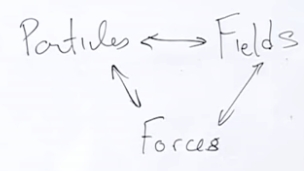
\includegraphics[width=0.5\textwidth]{ParticlesFieldsForces}
	\end{center}
\end{figure}

Consider two electric charges

\begin{align*}
E=&\int (e_1 \vec{E_1})^2 dV\\
E=&\int (e_2 \vec{E_2})^2 dV\\
E=&\int (e_1\vec{E_1}+e_2 \vec{E_2})^2 dV\\
=&\int \underbrace{(e_1\vec{E_1})^2}_\text{self energy}+ \underbrace{(e_2\vec{E_2})^2}_\text{self energy} + \underbrace{2e_1e_2\vec{E_1}.\vec{E_2}}_\text{interesting term}
\end{align*}

The first two terms represent self energy, which is includes in mass; the last term is proportional to the charges.
\begin{itemize}
	\item  If they are so far away that $\vec{E_1}$ is negligible near second charge there will be no perceptible effect.
	\item If the particles are close we will get a contribution from $\vec{E_1}.\vec{E_2}$. This turns out to be the Coulumb force. 
\end{itemize}

The force comes from the distortion of the field: this is a \emph{purely field view of forces}. If fields give rise to forces, and particles are quanta of fields, there must be a way to think of forces coming from particles.

Where do molecular forces come from? There are several mechanisms: we will focus on one. Imagine two protons and a single electron--Figure \ref{fig:2protons:electron}. Electron hops because of tunnelling.\footnote{Don't attempt to watch tunnelling! It is like any QM effect; watching ruins it.}

\begin{figure}[H]
	\caption[Molecular forces: two protons and a single electron]{Two protons and a single electron. Classically electron can't swap between Figures \ref{fig:2proton1Electrona} and \ref{fig:2proton1Electronb}, but QM allows it to tunnel.}\label{fig:2protons:electron}
	\begin{subfigure}{0.45\textwidth}
		\caption{Right hand protons is a long way from left: Schr\"odinger wave function for electron near left hand.} 
		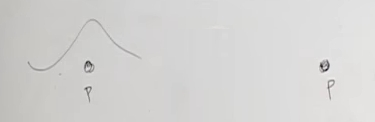
\includegraphics[width=0.9\textwidth]{2proton1Electrona}\label{fig:2proton1Electrona}
	\end{subfigure}
	\begin{subfigure}{0.45\textwidth}
		\caption{Protons closer together: Figure \ref{fig:2proton1Electrona} still possible, but so is this; they have the same energy.}
		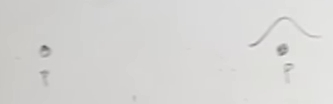
\includegraphics[width=0.9\textwidth]{2proton1Electronb}\label{fig:2proton1Electronb}
	\end{subfigure}
	\begin{subfigure}{0.45\textwidth}
		\caption{Effect of tunnelling}
		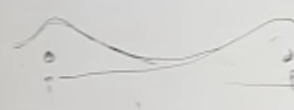
\includegraphics[width=0.9\textwidth]{2proton1Electronab}\label{fig:2proton1Electronab}
	\end{subfigure}
	\begin{subfigure}{0.45\textwidth}
		\caption{Energy as a function of distance between protons. Gradient in energy tries to move protons together, but Coulomb force tries to separate them; nett effect is a covalent bond.}
		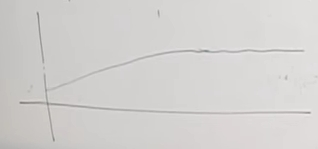
\includegraphics[width=0.9\textwidth]{2proton1ElectronEnergy}\label{fig:2proton1ElectronEnergy}
	\end{subfigure}
	\begin{subfigure}{0.45\textwidth}
		\caption{Electron exchange between protons. This lowers energy, leading to attraction.}
		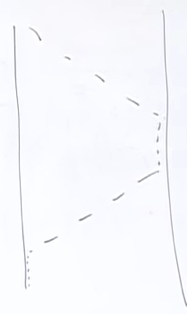
\includegraphics[width=0.9\textwidth]{2proton1ElectronHopping}\label{fig:2proton1ElectronHopping}
	\end{subfigure}
\end{figure}

Key ideas: 

\begin{itemize}
	\item adding wave functions leads to a lower energy state; energy is lowered by alternating between states;
	
	\item add 2nd electron, then total charge is zero, giving nett attraction; 

	\item so classically, add 2nd charge, lower energy (creates force) by distorting wave function;
	\item in QM, possibility of swapping between states lowers energy.
\end{itemize}
Can we think of Coulumb force in QM terms? Consider single proton and electron: proton interacts with electromagnetic field, whose quanta are photons.

\begin{itemize}
	\item Classically we solve field equations;
	\item In QM we think of emission and absorption of photons; this is what the Lagrangian tells us. One way to think of this is that the electron is a QM superposition of states: no photons, one with photon emitted,  one with two photons emitted, photon reabsorbed--Figure \ref{fig:2-1-electron-photons}. In Figure \ref{fig:2-1-electron-photons}, when electrons very far apart, energies just add. When they get closer, fields interact, or, in the language of Feynman diagrams, one electron absorbs electron emitted by the other--Figure \ref{fig:2-1-electron-photons-feynmann}.  Energy is no longer sum of energies of individual electrons, which gives rise to Coulomb force.
\end{itemize}

\begin{figure}[H]
	\caption{Emission and absorption of photons}
	\begin{subfigure}{0.45\textwidth}
		\caption{Electron absorbing and reabsorbing photons.}
		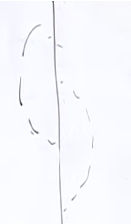
\includegraphics[width=0.9\textwidth]{2-1-electron-photons0}
	\end{subfigure}
	\begin{subfigure}{0.45\textwidth}
		\caption{The electron is a QM superposition of states}\label{fig:2-1-electron-photons}
		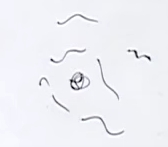
\includegraphics[width=0.9\textwidth]{2-1-electron-photons}
	\end{subfigure}
	\begin{subfigure}{0.45\textwidth}
		\caption{Two Electrons absorbing and reabsorbing photons.}\label{fig:2-1-second-electron-photons}
		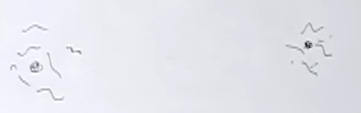
\includegraphics[width=0.9\textwidth]{2-1-second-electron-photons}
	\end{subfigure}
		\begin{subfigure}{0.45\textwidth}
		\caption{Feynman diagram of Electrons absorbing and reabsorbing photons. Sometimes one electron absorbs photon emitted to other.}\label{fig:2-1-electron-photons-feynmann}
		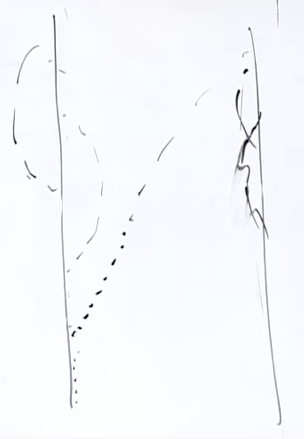
\includegraphics[width=0.9\textwidth]{2-1-second-electron-photons-feynman}
	\end{subfigure}
\end{figure}

In summary we have three ways of looking at forces:

\begin{itemize}
	\item laws such as Coulomb;
	\item classical field theory;
	\item exchange of particles. Every particle can be exchanged, so every particle produces a force. Not just 4 forces! 
\end{itemize}

The Standard Model is a mess. We don't understand why the particles are as they are. We understand some relationships. More types of particles than known relationships.

\begin{table}[H]
	\begin{center}
		\caption{Particles (Field symbol)}
		\begin{tabular}{|l|l|l|r|l|r|}\hline
			Name&Symbol&Type&Charge&B\#&Mass\\ \hline
			photon&$\gamma$ A&B&0&0&0 \\ \hline
			electron&$e+\pm \Psi_e\}$&F&-1&0&$0.15MeV$\\ \hline
			Quark&q&F&&$\frac{1}{3}$&\\ \hline
			down&q(Q) $\Psi_q$&F&$-\frac{1}{3}$&$\frac{1}{3}$&10meV\\ \hline
			up&&F&$\frac{2}{3}$&$\frac{1}{3}$&5meV\\ \hline
			strange&&F&$-\frac{1}{3}$&$\frac{1}{3}$&100meV\\ \hline
			charm&&F&$\frac{2}{3}$&$\frac{1}{3}$&1GeV\\ \hline
			bottom&&F&$-\frac{1}{3}$&$\frac{1}{3}$&5Gev\\ \hline
			top&&F&$\frac{2}{3}$&$\frac{1}{3}$&170Gev\\ \hline
		\end{tabular}
	\end{center}
\end{table}

Notes:\begin{enumerate}
	\item Particle and Field usually have the same name
	\item charge--electron is unit
	\item mass--unit is electron Volt--eV
	\item Proton has Baryon number 1.
	\item 3 families of quarks. Why?
\end{enumerate}

Figure \ref{fig:fep} depicts the way that electromagnetic processes emerge from a Lagrangian.

\begin{figure}[H]
	\caption{Electromagnetic processes emerge from a Lagrangian: $\mathcal{L}$: $e \Psi_e^\dagger \Psi_e A$}\label{fig:fep}
	\begin{subfigure}{0.45\textwidth}
		\caption{Fundamental electromagnetic process. Can rearrange.}\label{fig:fep1}
		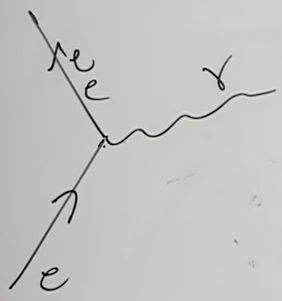
\includegraphics[width=0.9\textwidth]{2-1-em-process}
	\end{subfigure}
	\begin{subfigure}{0.45\textwidth}
		\caption{Fundamental electromagnetic process--exchange of particle.}\label{fig:fep2}
		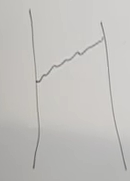
\includegraphics[width=0.9\textwidth]{2-1-em-process-feynman}
	\end{subfigure}
\end{figure}

Three quarks build baryons; two quarks build mesons--Table \ref{table:mesons}.
\begin{itemize}
	\item neutron: $ddu$ (slightly heavier)
	\item proton: $uud$ (self energy of energy partially offsets difference in quark masses)
\end{itemize}

Can we make an analogue of proton/neutron with strange quarks? Yes. E.g. $sdu$, $ssu$, $uus$ -- Strange baryons.


\begin{table}[H]
	\begin{center}
		\caption[Mesons: baryon number 0 - quark + anti-quark]{Mesons: baryon number 0 - quark + anti-quark. Note the two entangled pairs: $\frac{1}{\sqrt{2}}\big(\ket{\bar{u}u}\pm\ket{\bar{d}d}\big)$}\label{table:mesons}
		\begin{tabular}{|l|l|l|r|} \hline
			&Quarks&Charge&Mass\\ \hline
			$\pi^-$&$\bar{u}d$&-1&$\approx140 meV$ \\ \hline
			$\pi^+$&$u\bar{d}$&+1&$\approx140 meV$  \\ \hline
			$\pi^0$&$\frac{1}{\sqrt{2}}\big(\ket{\bar{u}u}+\ket{\bar{d}d}\big)$&0&$\approx140 meV$  \\ \hline
			$\eta$&$\frac{1}{\sqrt{2}}\big(\ket{\bar{u}u}-\ket{\bar{d}d}\big)$& 0&$\approx500 meV$ \\ \hline
			&$\bar{u}s$&-1& \\ \hline
			&$u\bar{s}$&+1& \\ \hline
			&$\bar{d}s$&0& \\ \hline
			&$d\bar{s}$&0& \\ \hline
			&$\bar{s}s$&0& \\ \hline
		\end{tabular}
	\end{center}
\end{table}

We also have strange mesons ($K-mesons$).


\section{Quantum Chromodynamics}

This is the theory of Quarks and gluons, and the things that they make.

\begin{defn}[Hadron]
	The things that Quarks and gluons make are called hadrons.
\end{defn}



\begin{defn}[Baryon]
	An object made of 3 quarks is called a baryon: they always have spin $\frac{1}{2}$, $\frac{3}{2},...$.
\end{defn}

\begin{defn}[Meson]
	An object made of quark plus antiquark is called a meson; mesons are quark-anti-quark pairs.
\end{defn}

\begin{defn}[Gluon]
	Electrically neutral stuff than holds quarks and antiquarks together.
\end{defn}

\subsection{Spin without group theory}
We start with the basic commutation relations:\cite{susskind2009particles}
\begin{align*}
	[L_x,L_y] =& i \hslash L_z\\
	[L_y,L_z] =& i \hslash L_x\\
	[L_z,L_x] =& i \hslash L_y
\end{align*}

In a previous set of lectures, \cite{susskind2009particles}:

\begin{itemize}
	\item we broke the symmetry by focusing on $L_z$.
	\item we can measure only one $L_i$ at a time.
	\item $L_i$ is quantized--$\hslash$.
\end{itemize}

\begin{table}[H]
	\begin{center}
		\caption{Spin multiplets: Spin $l$ denotes highest $L_z$.}
		\begin{tabular}{|c|l|l|} \hline
		$l$&Range of $L_z (Number=2l+1)$&Statistics\\ \hline
		$0$&$0$& Boson\\ \hline
		$\frac{1}{2}$&$\{-\frac{1}{2},\frac{1}{2}\}$& Fermion\\ \hline
		$1$&$\{-1,0,1\}$&Boson \\ \hline
		$\frac{3}{2}$&$\{-\frac{3}{2},-\frac{1}{2},\frac{1}{2},\frac{3}{2}\}$&Fermion \\ \hline
		$2$&$\{-2,-1,0,1,2\}$&Boson \\ \hline
		\end{tabular}
	\end{center}
\end{table}

\begin{table}[H]
	\begin{center}
		\caption[Ways to put two spin $\frac{1}{2}$ particles together]{Ways to put two spin $\frac{1}{2}$ particles together. Consider whether particles could disappear with violating conservation of angular momentum.}
		\begin{tabular}{|l|l|l|l|}\hline
			&$l$&$L_z$&Could disappear?\\ \hline
			$\ket{\uparrow\uparrow}$ &1&1&no--has $L_z$\\ \hline
			$\ket{\downarrow\downarrow}$&1&-1&no--has $L_z$ \\ \hline
			$\frac{1}{\sqrt{2}}(\ket{\uparrow\downarrow}+\ket{\downarrow\uparrow})$ &1&0&no--has $L_x$\\ \hline
			$\frac{1}{\sqrt{2}}(\ket{\uparrow\downarrow}-\ket{\downarrow\uparrow})$ &0&0&yes\\ \hline
		\end{tabular}
	\end{center}
\end{table}


\begin{table}[H]
	\begin{center}
		\caption{$3 \times \frac{3}{2}$ spins.}
		\begin{tabular}{|l|r|c|}\hline
			$\ket{\uparrow\uparrow\uparrow}$&$\frac{3}{2}$& \\ \hline
			$\ket{\downarrow\downarrow\downarrow}$&$-\frac{3}{2}$& \\ \hline
			$\ket{\uparrow\downarrow\downarrow}$,$\ket{\downarrow\uparrow\downarrow}$,$\ket{\downarrow\downarrow\uparrow}$&$\frac{1}{2}$&Three ways to do this\\ \hline
			$\ket{\uparrow\downarrow\downarrow}$,$\ket{\downarrow\uparrow\downarrow}$,$\ket{\downarrow\downarrow\uparrow}$&$-\frac{1}{2}$&Three ways to do this\\ \hline
		\end{tabular}
	\end{center}
\end{table}

\subsection{Isospin}

The natural energy of the nucleus is a few hundred meV, which comes from up and down quarks. To a first approximation, masses are close to each other, so they are analogous to spin. If we thinking of up and down quarks as isomorphic to up and down spins, we invent the concept of isospin.

\begin{itemize}
	\item $(\uparrow,\downarrow)$ gives ordinary spin;
	\item $(u,d)$ Isospin i.e.  $(p,n)$--makes Isotope.
\end{itemize}

Isospin isn't a precise symmetry of nature, as $u$ and $d$ have different masses and charges. But is is an approximate symmetry, for strong forces only.

The simplest object we can study is 3 quarks. We can make an object of isotopic spin $\frac{1}{2}$ or $\frac{3}{2}$--Table \ref{table:3quark}.

\begin{itemize}
	\item Assume that we can label quarks--${1,2,3}$
	\item Quarks are Fermions, so we need to anti-symmetrize. For example the proton should be: $\underbrace{d_1}_\text{isospin $\frac{1}{2}$}\underbrace{(u_2u_3-u_3u_2)}_\text{isospin 0}$.
	\item $\frac{1}{2}$: two states (isotopic spin doublet)
	\item $\frac{3}{2}$. $uuu$ and $ddd$, $\uparrow\uparrow\uparrow$, $\downarrow\downarrow\downarrow$. There are 4 states for isospin $\frac{3}{2}$--an isospin multiplet. NB, this $\Delta_\frac{3}{2}$ differs from the nucleon, as all spins are aligned. The $uud$ and $uud$ have an isospin component of $\frac{1}{2}$, even though total isotopic spin is $\frac{3}{2}$.
\end{itemize}

\begin{table}[H]
	\begin{center}
		\caption[Simplest object we can study is 3 quarks.]{Simplest object we can study is 3 quarks. We can make an object of isotopic spin $\frac{1}{2}$ or $\frac{3}{2}$.}\label{table:3quark}
		\begin{tabular}{|c|c|c|c|r|r|}\hline
			Isospin&Quarks&Spin&Name&Charge&Mass\\ \hline
			$\frac{1}{2}$&$duu$&$\frac{1}{2}$&proton&$+1$&940meV\\ \hline
			$\frac{1}{2}$&$udd$&$\frac{1}{2}$&neutron&0&940meV\\ \hline
			$\frac{3}{2}$&$uuu$&$\frac{3}{2}$&$\Delta_\frac{3}{2}$&$+2$&1200meV\\ \hline
			$\frac{3}{2}$&$ddd$&$\frac{3}{2}$&$\Delta_\frac{3}{2}$&-1&1200meV\\ \hline
			$\frac{3}{2}$&$uud$&$\frac{3}{2}$&$\Delta_\frac{3}{2}$&+1&1200meV\\ \hline
			$\frac{3}{2}$&$udd$&$\frac{3}{2}$&$\Delta_\frac{3}{2}$&0&1200meV\\ \hline
		\end{tabular}
	\end{center}
\end{table}

Figure \ref{fig:decay:dalta} shows the decay of $\Delta_\frac{3}{2}$.

\begin{figure}[H]
	\begin{center}
		\caption[Decay of a $\Delta_\frac{3}{2}$]{Decay of a $\Delta_\frac{3}{2}$. Quarks can't go off on their own, so we need a quark-antiquark pair to balance. $\Delta_\frac{3}{2}\rightarrow p +\pi^+$: there is enough energy in $\Delta_\frac{3}{2}$ to create the $\pi^+$.}\label{fig:decay:dalta}
		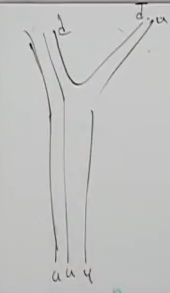
\includegraphics[width=0.6\textwidth]{2-2-Delta-decay}
	\end{center}
\end{figure}

\subsection{Quantum Chromodynamics}

We have a problem: $uuu$ represents three Fermions whose spins are all in the same direction, which violates the Pauli Exclusion Principle. Quarks must have another property: the three quarks must have a label which is hidden from view and not apparent in experiments. This is called "colour", a totally arbitrary name which has nothing to do with ordinary colour: it is just a name. Values are Red, Blue, and Green. The important thing is that they have precisely 3 different values. The  $\Delta_\frac{3}{2}$ is important because of having 3 u or d. For proton we need to [anti?]symmetrize: $\ket{d_R u_G u_B}+...$

What holds quarks together? Electrons use protons / electromagnet field. Quarks use gluons: spin 1, so same polarization states, massless, but one big difference(later), and they jump back and forth. Quarks emit and absorb gluons.

The fundamental electromagnetic process is depicted in Figure \ref{fig:fep1}. A photon is similar to electron and positron, e.g. it has the same properties: a sufficiently energetic photon can decay into an electron and positron pair.

\begin{figure}[H]
	\caption{Gluons}
	\begin{subfigure}{0.45\textwidth}
		\caption{Introducing the gluon}
		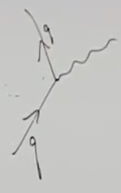
\includegraphics[width=0.9\textwidth]{2-2-gluon1}
	\end{subfigure}
	\begin{subfigure}{0.45\textwidth}
		\caption{A gluon behaves a bit like a quark-antiquark pair: this the gluon as a fictitious quark-antiquark pair}
		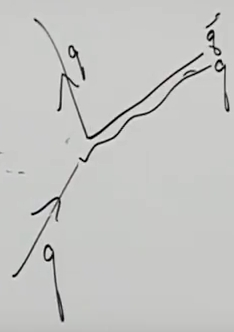
\includegraphics[width=0.9\textwidth]{2-2-gluon2}
	\end{subfigure}

\end{figure}

There are 9 possible gluons (we will see later that there are actually only 8--Section \ref{sec:3:3:8}):
\begin{align*}
\begin{pmatrix}
R\bar{R}&R\bar{G}&R\bar{B}\\
G\bar{R}&G\bar{G}&G\bar{B}\\
B\bar{R}&B\bar{G}&B\bar{B}
\end{pmatrix}
\end{align*}

Gluons can interact with each other--Figure \ref{2-2-gluon6}.
\begin{figure}[H]
	\caption{The basic vertices of QCD}
	\begin{subfigure}{0.45\textwidth}
		\caption{Red quark changes to green: analogous to process with photon.}
		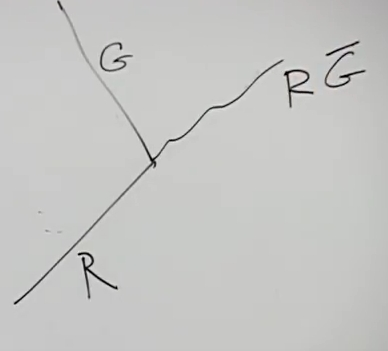
\includegraphics[width=0.9\textwidth]{2-2-gluon3}
	\end{subfigure}
	\begin{subfigure}{0.45\textwidth}
		\caption{Red quark changes to green, using fictitious quark-antiquark pair}
		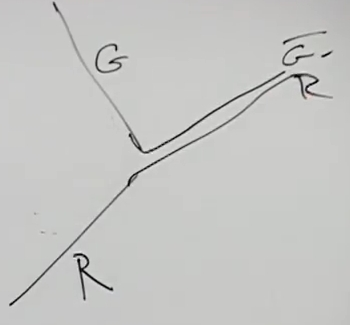
\includegraphics[width=0.9\textwidth]{2-2-gluon4}
	\end{subfigure}
	\begin{subfigure}{0.45\textwidth}
		\caption{Second basic vertex, which has no analogue for photons. Fictitious quark-antiquark pairs represent gluons. This process makes QCD more complex and more interesting.}\label{2-2-gluon5}
		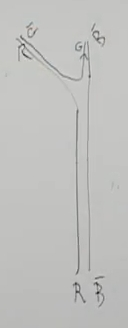
\includegraphics[width=0.9\textwidth]{2-2-gluon5}
	\end{subfigure}
	\begin{subfigure}{0.45\textwidth}
		\caption{Second basic vertex, redrawn with gluons, instead of fictitious quark-antiquark pairs. Use Figure \ref{2-2-gluon5} to determine which combinations don't break any lines.}\label{2-2-gluon6}
		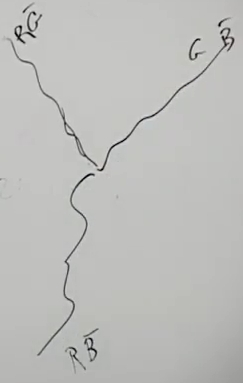
\includegraphics[width=0.9\textwidth]{2-2-gluon6}
	\end{subfigure}
\end{figure}

Photons cannot exchange photons, but gluons can exchange gluons, which means that there are \emph{forces between gluons}--Figure \ref{fig:quarks:gluons:forces}. Two waves of gluons can deform each other; different parts of one wave of gluons can deform each other: the dynamics is non-linear.

\begin{figure}[H]
	\caption{Photons cannot exchange photons, but gluons can exchange gluons.}\label{fig:quarks:gluons:forces}
	\begin{subfigure}{0.45\textwidth}
		\caption{Force between quarks}
		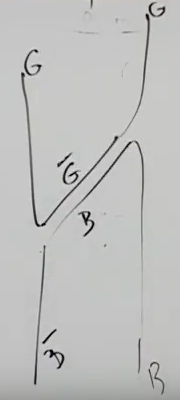
\includegraphics[width=0.9\textwidth]{2-2-gluon7}
	\end{subfigure}
		\begin{subfigure}{0.45\textwidth}
		\caption{Force between gluons}
		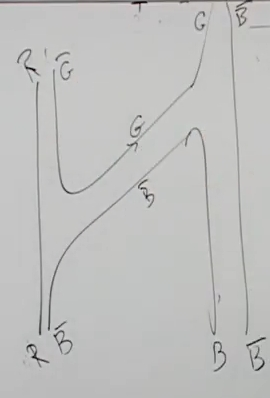
\includegraphics[width=0.9\textwidth]{2-2-gluon8}
	\end{subfigure}
\end{figure}

The only rule is: follow the lines and, if the line turn around, change particle to antiparticle.

Figure \ref{fig:2-2-mass1} shows that masses of objects are frequency dependent. In the same sense, masses of quarks depend on frequency.
\begin{itemize}
	\item  Move slowly and we drag gluons with quark.
	\item Move at high frequency, we drag $m$ (quark) only
\end{itemize}

\begin{figure}[H]
	\caption[Mass (quark) with squishy thing attached]{Mass with squishy thing attached. If we move slowly we drag attachment, fast we just move mass. The concept of mass of quark is ambiguous: normally we mean the high frequency mass.}\label{fig:2-2-mass1}
	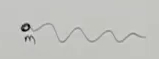
\includegraphics[width=0.8\textwidth]{2-2-mass1}
\end{figure}


\section{Group Theory I: Group Representations}

Rotations in space act on vectors: they rotate one vector to another. Rotations can be combined: they form a non-Abelian group. Figure \ref{fig:2-3-paramerize-rotation} depicts one way to parametrize rotation--axis $\vec{n}$ and angle $\theta$. Since $\vec{n}$ can be parametrized by two angles, latitude and longitude, we need 3 angles in total.

\begin{figure}[H]
	\begin{center}
		\caption{Parametrize rotation: axis $\vec{n}$ and angle $\theta$}\label{fig:2-3-paramerize-rotation}
		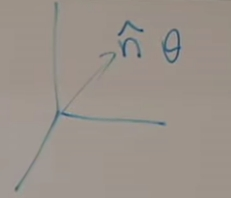
\includegraphics[width=0.8\textwidth]{2-3-paramerize-rotation}
	\end{center}
\end{figure}

Colour is a representation of the rotation group.

How do we construct a matrix representation of rotations? 

\begin{align*}
	\sum_j R_{ij}(\theta,\vec{n})V_j=&V_i^\prime \\
	R \vec{V} =&\vec{V^\prime} \text{. Now if $R$ is a rotation, it doesn't change length}\\
	\forall \vec{V} \; \sum_i V_i^2 =& \sum_i (V_i^\prime)^2\\
	\sum_{i,j,k} R_{ij} R_{ik} V_j V_k =& \sum_i V_i V_i \text{, i.e.}\\
	\sum_{i} R_{ij} R_{ik} =& \delta_{j,k} \text{, or}\\
	R^T R =& I
\end{align*}

There are 3D representations of the rotation group. Can we think of them being related to quantum states? Spin describes angular momentum. A spin 1 particle (vector boson) can be described by a column vector containing amplitudes for the various components of spin. What about spin $\frac{1}{2}$ particle?

\begin{align*}
	\begin{pmatrix}
		1\\
		0
	\end{pmatrix}=& \ket{u}\\
	\begin{pmatrix}
		0\\
		1
	\end{pmatrix}=& \ket{d}\\
	\begin{pmatrix}
		\alpha_1\\
		\alpha_2
	\end{pmatrix}=& \alpha_1 \ket{u} + \alpha_2 \ket{v} \text{, where $\alpha_1^2+\alpha_2^2=1$}
\end{align*}

We can represent rotation by a $2\times2$ matrix acting on spinors.

\begin{align*}
	\begin{pmatrix}
		U_{11}&U_{12}\\
		U_{21}&U_{22}
	\end{pmatrix} 	\begin{pmatrix}
		\alpha_1\\
		\alpha_2
	\end{pmatrix} =& \begin{pmatrix}
		\alpha^\prime_1\\
		\alpha^\prime_2
	\end{pmatrix} \text{{. Now if}}\\
	\alpha^*_1 \alpha_1 + \alpha^*_2 \alpha_2 =& 1 \text{ we want}\\
	(\alpha^\prime_1)^* (\alpha^\prime_1) + (\alpha^\prime_2)^* (\alpha^\prime_2) =& 1 \text{, which gives}\\
	(U^T)^* U =& I \text{, which can be written} \\
	U^\dagger U =& I \numberthis \label{eq:unitary:2}
\end{align*}

$U$ has 8 degrees of freedom, but (\ref{eq:unitary:2}) imposes 4 constraints, yielding 4 degrees of freedom. But 3D rotations only have 3 degrees of freedom. We set $\det(U)=1$ to give a 2 parameter group, $SU(2)$

\begin{defn}[$U(N)$]
	The group of unitary $N\times N$ matrices.
\end{defn}

\begin{defn}[$SU(N)$]
	The subgroup of $U(N)$ with determinant 1.
\end{defn}

\begin{thm}[$SU(N)$]
	Any small rotation in $SU(N)$ can be expressed as:
	\begin{align*}
		U =& I + i \epsilon M \text{, where $M$ is a linear combination of the Pauli matrices $\sigma_i$}\\
		\sigma_x =& \begin{pmatrix} \numberthis \label{eq:pauli:x}
		0&1\\
		1&0
		\end{pmatrix}\\
		\sigma_y =& \begin{pmatrix} \numberthis \label{eq:pauli:y}
		0&-i\\
		i&0
		\end{pmatrix}\\
		\sigma_z =& \begin{pmatrix} \numberthis \label{eq:pauli:z}
		1&0\\
		0&-1
		\end{pmatrix}
	\end{align*}
\end{thm}

\begin{proof}
	\begin{lemma}[Determinant and Trace]\label{lemma:det:Tr}
		\begin{align*}
		\det( I + i \epsilon M) =& 1 + i\epsilon(Tr(M)) + O(\epsilon^2)
		\end{align*}
	\end{lemma}
	\begin{proof}
		TBP
	\end{proof}
	\begin{lemma}[Traceless Hermitian $2\times2$ matrix]\label{lemma:traceless:22}
		Any traceless Hermitian $2\times2$ matrix can be written as a linear combination of the Pauli  matrices.
	\end{lemma}
	\begin{proof}
		content...
	\end{proof}

	For small rotations:
	\begin{align*}
	U =& I + i \epsilon M \text{. Now}\\
	I =&U U^\dagger \text{ from (\ref{eq:unitary:2}), so}\\
	=& (I + i \epsilon M)(I - i\epsilon M^\dagger) \text{, which expands to}\\
	=& I + i \epsilon(M - M^\dagger) - \epsilon^2 M^\dagger \text{. If we discard $O(\epsilon^2)$}\\
	M - M^\dagger =& 0 \text{, i.e. M is Hermitean.}
	\end{align*}
	We also need U to be unimodular:
	\begin{align*}
	1=&\det(U)\\
	=& \det( I + i \epsilon M) \text{. Now, using Lemma \ref{lemma:det:Tr}}\\
	=& 1 + i\epsilon(Tr(M)) \text{, whence:}\\
	Tr(M) =&0
	\end{align*}
	
	The result follows from Lemma \ref{lemma:traceless:22}.
	
\end{proof}

State of quark can be Red, Green, or Blue. 
\begin{align*}
	\begin{pmatrix}
		\alpha_1\\
		\alpha_2\\
		\alpha_3
	\end{pmatrix} \quad	\begin{pmatrix}
	\Psi_r\\
	\Psi_g\\
	\Psi_b
	\end{pmatrix}
\end{align*}

We can multiply by a member of $SU(3)$. These have $18-9-1=8$ degrees of freedom. Every term in Lagrangian needs to be invariant under $SU(3)$.  


\section{Group Theory – II}

\subsection{Group Theory}
$SU(2)$ is not exactly the same as 1D rotations: there is a $2\rightarrow1$ correspondence, not  $1\rightarrow1$, since $-U$ and $U$ correspond to the same rotation. This is why the electron wave function is called a doublet.

Generators are closely connected to infinitesimal elements. If you know structure of generators you can work out the whole structure. Generators let us figure out conservation laws.

\begin{align*}
	U =& I + i \epsilon T\\
	I =& U^\dagger U + 1\\
	=& I + i\epsilon(T - T^\dagger) - \epsilon^2 T T^\dagger\\
	T =& T^\dagger \text{. Hermitian -- observable}\\
	\det(U) =& 1\\
	\implies&\\
	Tr(t)=&0
\end{align*}

Since the 3D rotation group has three parameters, the Ts span a 3D space. See (\ref{eq:pauli:x}), (\ref{eq:pauli:y}), and (\ref{eq:pauli:z}). Can figure out generators from commutation rules.

In SU(3) we have $3\times3$ matrices, so $3\times3\times2=18$ real components; the matrix being unitary imposes 9 constraints, and unimodularity imposes one more, whence there are $18-9-1=8$ degrees of freedom.

Combining representations to form new representations. E.g. we might compose spins to make a composite. E.g. combine 2 spin $\frac{1}{2}$ objects. We have 4 possible states: a basis in that space can be thought of as a spin 0 object plus 3 spin 1 objects. We can make ${-1,0,+1}$, but the zero can be done in 2 ways: so one of the zero spins must not be part of the spin 1 multiplet, it can only be spin 0 (ortho- and para-hydrogen).

\subsection{Representations of $SU(3)$.}

Triplet: $3\times3$ matrix acting on RGB vector, mixing up states, transforming to a quantum superposition.

There are 3 important representations: 

\subsubsection{The \bfseries{3}}

\begin{align*}
	\begin{pmatrix}
		q_r\\
		q_g\\
		q_b
	\end{pmatrix} \text{ field operator--creation}
\end{align*} 

\subsubsection{$\bar{3}$}

Antiquarks, represented by complex conjugates (not Hermitian conjugates)

\begin{align*}
	U q =& q^\prime\\
	U^* q^* = q^\prime& 
\end{align*}

Electron and positron are complex conjugate representations of $U(1)$. ($e^{i\theta}\psi_e \rightarrow e^{-i\theta}\psi_p$).

Generators of $\bm{\bar{3}}$ are negatives of generators of {\bfseries 3}, so they carry negative colour.

\subsubsection{$3 \otimes 3$}\label{sec:3:3:8}

Combine two quarks ${RR, RG, RB,...}$

\begin{align*}
	3 \otimes 3 =& \underbrace{\bar{3}}_\text{combine antisymmetrically} \oplus \underbrace{6}_\text{combine symmetrically}\\
	3 \otimes \bar{3} =& \underbrace{1}_\text{singlet: $R\bar{R}+G\bar{G}+B\bar{B}$} \oplus \underbrace{8}_\text{8 dimensional representation--generators!}
\end{align*}

\begin{align*}
3 \otimes 3 \otimes 3 =& (3 \otimes 3) \otimes 3\\
=& \big(\bar{3} \oplus 6 \big) \otimes 3\\
=& \bar{3}   \otimes 3 + 6 \otimes 3\\
=& \underbrace{1}_\text{anti-symmetrized superposed R, G, B} \oplus 8 \oplus 8 \oplus 10
\end{align*}

Gluon behaves a quark-antiquark under colour symmetry: it transforms under the 8 (octet).

\subsection{Quantum Chromodynamics (resumed)}

\begin{table}[H]
	\begin{center}
		\caption{Postulates of QCD.}\label{table:postulates:QCD}
		\begin{tabular}{|l|c|p{8cm}|} \hline
			Particle&Group&Remarks \\ \hline
			Quark&{\bfseries 3}& \\ \hline
			Antiquark&$\bm{\bar{3}}$& \\ \hline
			qluon&{\bfseries 8}&$\bm{3}\otimes\bm{3}=\bm{8}\oplus\bm{1}$, but the $\bm{1}$ does not exist in nature. It also doesn't mix with other components, so it is consistent to throw it away \\ \hline
			Free particles&{\bfseries 1}&All observable particles transform as singlets: quark+antiquark, or 3 quarks.\\ \hline
			&&Gluons play the same role in QCD as photons in QED, sourced from the 8 generators--Figure \ref{fig:2-4-quark-gluon-field}. Just as electric field of two particles has lower energy if total charge zero, gluon fields have lowest energy if total colour zero. But coupling constant higher, which is why we don't see free quarks.\\ \hline
		\end{tabular}
	\end{center}
\end{table}

What if we combine gluons together, or gluons with quarks?

\begin{defn}[Glueball]
	Combine two gluons. $\bm{8} \otimes \bm{8} = \bm{63} \oplus \bm{1}$ -- 2 gluons. The singlet is known as a glueball.
\end{defn}

There are 3 kinds of Hadrons:
\begin{itemize}
	\item Baryons
	\item Mesons
	\item Glueballs
\end{itemize}

$SU(3)$ singlets also give integer charge, as phases cancel.

Back to $SU(2)$. We have $\Psi_i$. To make two particles act twice: $\Psi_i\Psi_j$, or $\Psi_i\Phi_j$(two different particles). We have a tensor-like object, having repeated indices.

\begin{align*}
	\begin{pmatrix}
		.&.&.&.\\
		.&.&.&.\\
		.&.&.&.\\
		.&.&.&.
	\end{pmatrix} 	\begin{pmatrix}
\Psi_u\Phi_u\\
\Psi_u\Phi_d\\
\Psi_d\Phi_u\\
\Psi_d\Phi_d
\end{pmatrix} 
\end{align*}
 The operator mixes things up, but we find
\begin{align*}
    \Psi_u\Phi_d-\Psi_d\Phi_u \text{, unchanged --singlet}	
\end{align*}
The next 3 mix among themselves and behave like a spin 1 object, the {\bfseries 3}.
\begin{align*}
	\begin{cases}
		\Psi_u\Phi_d+\Psi_d\Phi_u\\
		\Psi_u\Phi_u\\
		\Psi_d\Phi_d
	\end{cases}
\end{align*}

In the right basis:
\begin{align*}
	\begin{pmatrix}
		1&0&0&0\\
		0&.&.&.\\
		0&.&.&.\\
		0&.&.&.
	\end{pmatrix}
\end{align*}



The 8 gluons aren't neutral, as they have colour. The carry large amounts of energy, and don't appear as free particles. Gluons can interfere with each other, which is why QCD is more complicated than QED--see Figure \ref{fig:QCD:QED}.
 
\begin{figure}[H]
	\caption{Why QCD is more complicated than QED}\label{fig:QCD:QED}
	\begin{subfigure}{0.45\textwidth}
		\caption[Quark surrounded by Gluon Field]{Quark surrounded by Gluon Field: there are 8 such fields, which transform according to the {\bfseries 8}.}\label{fig:2-4-quark-gluon-field}
		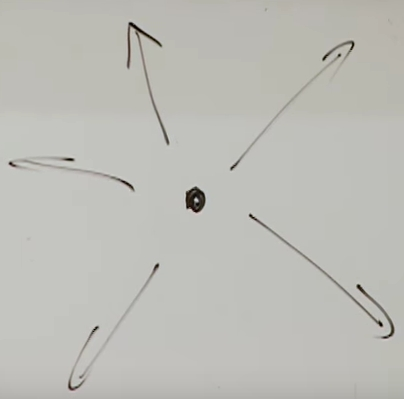
\includegraphics[width=0.9\textwidth]{2-4-quark-gluon-field}
	\end{subfigure}
	\begin{subfigure}{0.45\textwidth}
		\caption{If Figure \ref{fig:2-4-quark-gluon-field} were an electromagnetic field, field lines would not attract or repel each other. In QCD they have colour, so they attract each other and form tubes.}
		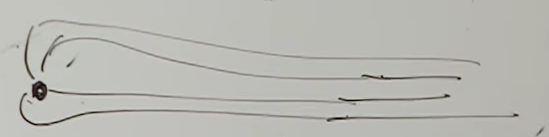
\includegraphics[width=0.9\textwidth]{2-4-quark-gluon-field-tubes}
	\end{subfigure}
	\begin{subfigure}{0.45\textwidth}
		\caption{Tube linking quark and anti-quark-fluxoid. There is a uniform field, no matter how far particles separated.}
		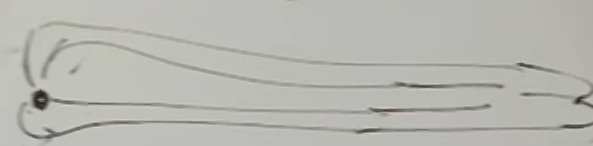
\includegraphics[width=0.9\textwidth]{2-4-quark-gluon-field-tubes-QAQ}
	\end{subfigure}
	\begin{subfigure}{0.45\textwidth}
		\caption{Fluxoid. There is a uniform energy per unit length, so force increases as tube stretches. Unless flux tube ends at a quark/antiquark, energy is infinite.}
		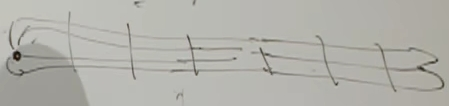
\includegraphics[width=0.9\textwidth]{2-4-quark-gluon-field-tube-uniform-energy}
	\end{subfigure}
	\begin{subfigure}{0.45\textwidth}
		\caption{If meson has enough energy, tube may break, using quark-antiquark pair from vacuum. This forms a jet.}
		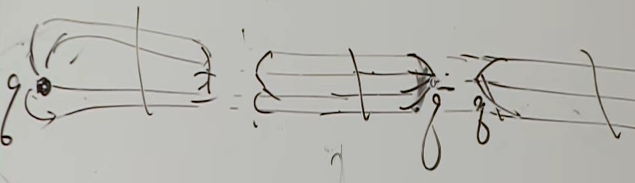
\includegraphics[width=0.9\textwidth]{2-4-split-meson}
	\end{subfigure}
\end{figure}

QCD is a gauge field.

\begin{defn}[Gauge field]
	A gauge field is any theory where conserved quantities are coupled to a Maxwell-like field. They are always based on symmetries.
\end{defn}

Charges linked to lines of force. In Figure \ref{fig:2-4-quark-gluon-field}, fields lines must end on charge means charge conserved, which related to symmetry.

\section{Gauge Fields and Symmetry}

\subsection{Gauge Fields and Symmetry}

Just about all of nature is controlled by gauge theories.

The first and simplest gauge theory is Maxwell's theory. This has six components, the electric and magnetic fields, which are generated from a potential $A_\mu=(A_0,\vec{A})$.
\begin{itemize}
	\item  $A_0$ is the electric potential: $F_i=e \frac{\partial A_0}{\partial x_i}$.
	\item Electric field $\vec{E}=\nabla A_0$.
	\item Magnetic field $\vec{B}=\nabla \times \vec{A}$
\end{itemize}

\begin{figure}[H]
	\caption[Electromagnetic waves, illustrating Polarization.]{Electromagnetic waves. Polarization is in direction of electric field.}
	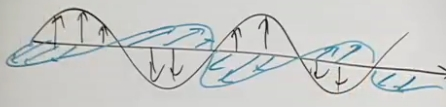
\includegraphics[width=0.8\textwidth]{2-5-EM-field}
\end{figure}

The essence of a gauge theory: in Maxwell-like theories, with electric-like and magnetic-like fields, if gauge field is weakly coupled (interactions between parts don't interfere with each other), motion of a gauge field is exactly the same as a light wave; it moves at the speed of light unless something interferes.

Gauge theories  always have conserved quantities, hence symmetries. Colour is an example.
\begin{itemize}
	\item  We'll call the potential $A_{ij}$, which transforms under $SU(3)$.
	\item Symmetry: $U_{ij} q_j = q^\prime_i$ (indexed over colour).
	\item The $q_i$ form a representation of $SU(3)$, known as the fundamental representation.
	\item The antiparticles are represented $U^*_{ij} q^*_j = q^(\prime_i*)$. We have two distinct representations, {\bfseries 3} and $\bm{\bar{3}}$.
	\item  $A_{ij}$ has same structure as $\bar{q}_i q_j$.
	\item $A_{ij}$ transforms like quark/antiquark, and  trace vanished (adjoint representation).
	\item $A_{ij}$ transforms according to $SU(3)$  (unlike photon--not charge).
\end{itemize}

\begin{figure}[H]
	\caption{Basic interactions of gauge theory}
	\begin{subfigure}{0.45\textwidth}
		\caption{i becomes j by emitting a quantum of field $A_{ji}$}
		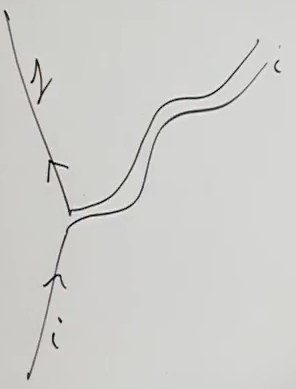
\includegraphics[width=0.9\textwidth]{2-change-charge}
	\end{subfigure}
	\begin{subfigure}{0.45\textwidth}
		\caption{Interaction with gluons only: they exert forces that photons don't.}
		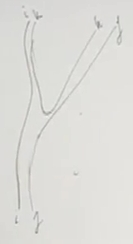
\includegraphics[width=0.9\textwidth]{2-5-gluon-gluon.jpg}
	\end{subfigure}
\end{figure}

\subsection{Strong and Weak Interactions}

A Gauge theory also needs a coupling constant, analogous to the charge of the electron (amplitude for emitting photon). EM is weak: probability of emission is $\frac{1}{137}$.

Set $c=1$, $\hslash=1$, then energy is in units of $\frac{1}{T}$: $1eV^{-1}=10^{-7}M$.

\subsubsection{Strong and Electromagnetic Interactions}

Table \ref{table:ems} compares various properties of the Strong and Electromagnetic Interactions.

\begin{table}[H]
	\begin{center}
		\caption{Electromagnetic and strong}\label{table:ems}
		\begin{tabular}{|l|r|r|} \hline
			&Atom&Hadron \\ \hline
			$\alpha$&$\frac{1}{137}$&\\ \hline	
			Diameter atom&$10^{-10}M$&$10^{-15}M$ \\ \hline
			Transit time &$10^{-18}S$&$10^{-23}S$\\ \hline
			Orbital time &$10^{-18}S$&$10^{-23}S$\\ \hline
			Decay time (from $1^{st}$ excited state)&$10^{-9}S$&$10^{-23}S$\\ \hline
		\end{tabular}
	\end{center}
\end{table}

Times for Hadrons less spread out: QCD version of $\alpha$ much closer to 1 ($\frac{1}{5}$). This is why strong interactions are called strong.

\subsubsection{Weak Interactions}

There is another set of interactions that are characterized by being quite slow. Table \ref{table:ex:weak} gives examples.

\begin{table}[H]
	\begin{center}
		\caption{Examples of Weak decay}\label{table:ex:weak}
		\begin{tabular}{|l|l|p{6cm}|}\hline
			$n \rightarrow e + p +\bar{\nu}$&12 minutes&Barely enough energy: 940meV $\rightarrow$ 939meV + 0.5meV, but this isn't enough to explain the slowness.\\ \hline
			$\pi^- \rightarrow e^- + \bar{\nu} $&$10nS$&Plenty of energy, but still slow.\\ \hline
			$\pi^+ \rightarrow e^+ + \nu $&&\\ \hline
		\end{tabular}
	\end{center}
\end{table}

These are very slow: clearly something else is going on! Table \ref{tab:QCD:rows} is relevant. \begin{itemize}
	\item Colour symmetry, $SU(3)$, operates on rows; a $u$ remains a $u.$
	\item We introduce a new gauge symmetry, $SU(2)$ operating horizontally: $u\leftrightarrow d$;  $c\leftrightarrow s$;  $t\leftrightarrow b$.
\end{itemize}

\begin{table}[H]
	\begin{center}
		\caption{Quarks: Colour symmetry operates on first three rows, not on columns}\label{tab:QCD:rows}
		\begin{tabular}{|c|c|c|c|} \hline
			&u d&c s&t b \\ \hline
			red&x x&x x&x x\\ \hline
			green&x x&x x&x x\\ \hline
			blue&x x&x x&x x\\ \hline
			leptons&$\nu_e$ e&$\nu_\mu$ $\mu$&$\nu_\tau$ $\tau$\\ \hline
		\end{tabular}
	\end{center}
\end{table}

The last row deals with Leptons. They appear in an order that depends on the charge difference: $u-d=\nu_e-e$

We postulate a gauge boson that combines particle and antiparticle, and apply it to leptons, e.g, $e \bar{\nu_e}$. We call this gauge boson, $W$:

 \begin{itemize}
 	\item $e \bar{\nu_e}\leftrightarrow W^- \leftrightarrow d\bar{u}$
 	\item $e^+ \nu_e\leftrightarrow W^+ \leftrightarrow \bar{d}u$
 \end{itemize}

This is sometimes known as the flavour symmetry.

Imagine that W is like photons or gluons, so it behaves as shown in Figure \ref{fig:W:photon:fluon}.

\begin{figure}[H]
	\caption{W are like photons or gluons}\label{fig:W:photon:fluon}
	\begin{subfigure}{0.2\textwidth}
		\caption{$e \rightarrow\nu + W^-$}\label{fig:2-5-W1}
		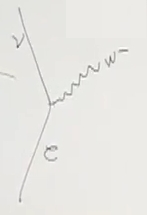
\includegraphics[width=0.9\textwidth]{2-5-W1}
	\end{subfigure}
	\begin{subfigure}{0.2\textwidth}
		\caption{$d \rightarrow u + W^-$}
		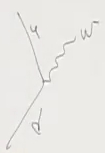
\includegraphics[width=0.9\textwidth]{2-5-W2}
	\end{subfigure}
	\begin{subfigure}{0.2\textwidth}
		\caption{$s \rightarrow c + W^-$}
		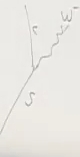
\includegraphics[width=0.9\textwidth]{2-5-W3}
	\end{subfigure}
	\begin{subfigure}{0.2\textwidth}
		\caption{$W^+$ and $W^-$ are antiparticles, so we can redraw \ref{fig:2-5-W1}}
		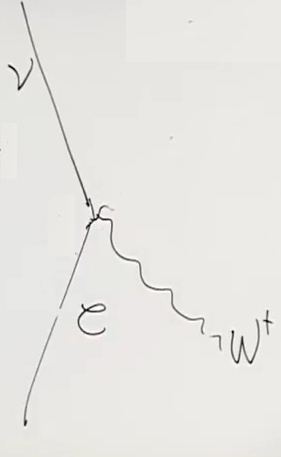
\includegraphics[width=0.9\textwidth]{2-5-W4}
	\end{subfigure}
\end{figure}

\begin{figure}[H]
	\caption{Examples of W boson mediated decays}
	\begin{subfigure}{0.30\textwidth}
		\caption{Pion decay (electron, muon, tau, and associated neutrino)}
		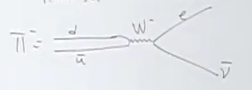
\includegraphics[width=0.9\textwidth]{2-5-pion-decay}
	\end{subfigure}
	\begin{subfigure}{0.30\textwidth}
		\caption{Muon decay}
		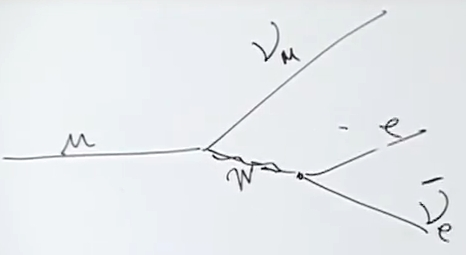
\includegraphics[width=0.9\textwidth]{2-5-muon-decay}
	\end{subfigure}
	\begin{subfigure}{0.30\textwidth}
		\caption{Neutron decay. W doesn't have enough energy to make muon, unless we hit neutron really hard.}
		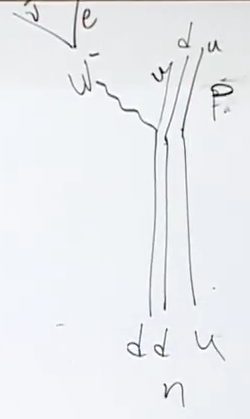
\includegraphics[width=0.9\textwidth]{2-5-neutron-decay}
	\end{subfigure}
\end{figure}

NB: can violate conservation for a very short time.

Why so slow? Coupling constant?(No)

\section{The Weak Interaction}

\subsection{Why is the weak interaction so slow?}

In Figure \ref{tab:QCD:rows} we have three symmetries: $SU(3) \otimes SU(2) \otimes U(1)$. We say that the Standard Model is a gauge theory based on  $SU(3) \otimes SU(2) \otimes U(1)$.

\begin{table}[H]
	\begin{center}
		\caption{Coupling Constants}
		\begin{tabular}{|l|l|l|} \hline
			Group&Coupling Constant&Remarks \\ \hline
			$U(1)$&e& \\ \hline
			$SU(3)$&$g_s \approxeq 1$& \\ \hline
			$SU(2)$&$g_w$& \\ \hline
		\end{tabular}
	\end{center}
\end{table}



\begin{figure}[H]
	\caption{Possible fates for q W boson}
	\begin{subfigure}{0.6\textwidth}
		\caption{Decay of a neutron. The $W$ line is the \emph{propagator}}\label{fig:2-6-W1}
		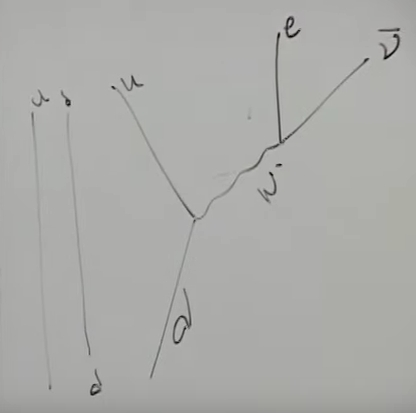
\includegraphics[width=0.8\textwidth]{2-6-W1}
	\end{subfigure}
	\begin{subfigure}{0.4\textwidth}
		\caption{A different fate for a W Boson: re-absorption}\label{fig:absorption:W:boson}
		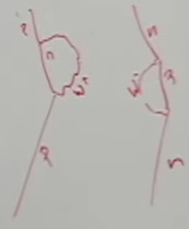
\includegraphics[width=0.8\textwidth]{2-6-W2}
	\end{subfigure}
\end{figure}

The Propagator is a function of proper time between two points: $\Delta(ds)$, the distance between the two points. $g_w^2 \Delta$

\begin{figure}[H]
	\caption[Propagator $\Delta(ds)$ as a function of distance.]{Propagator $\Delta(ds)$ as a function of distance. Black line is for zero mass, $\frac{1}{ds}$, red for non-zero.}
	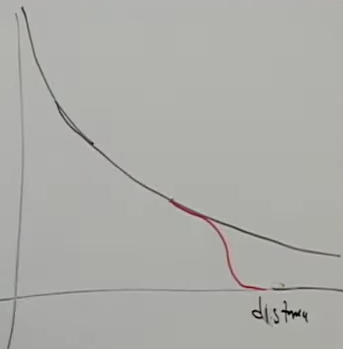
\includegraphics[width=0.8\textwidth]{2-6-propagator}
\end{figure}

Where does $\Delta$ decrease suddenly? Choose units where $c=\hslash=1$:
\begin{align*}
	[m] =& [E]\\
	=& [L^{-1}]\\
	=& [P]\\
	distance \propto & \frac{1}{L} \text{, in fact:}\\
	distance \approxeq & \frac{\hslash}{mc} \text {, Compton wavelength}
\end{align*}

$\Delta^2$ is probability particle can get that far.

In an experiment, we know the momenta. We can think of propagator as function of position, or momentum--using Fourier transform:
\begin{align*}
\tilde{\Delta}(k_w)=\frac{1}{k_w^2+m_w^2} \numberthis \label{eq:Delta}
\end{align*}
 $\tilde{\Delta}(k_w)$ will have its biggest value when $k_w=0$, so the most likely thing is to emit a low momentum W, which costs an amplitude of $\frac{1}{m_w^2}$. Amplitude for emitting $W$ and converting to electron plus neutrino is $\frac{g_w^2}{m_w^2}$: weak interactions are made weak because the mass of the W is large--about 100 protons! Probability is $\frac{g_w^4}{m_w^4}$.
 
 W is produced virtually. From the energy-time uncertainty principle, energy conservation can be violated briefly: $\delta T \delta E<\hslash$. There is not enough energy in neutron to make W, but it can briefly make a W, which must be destroyed again.\footnote{I have left out a discussion where Prof Susskind shows that trying to watch the virtual particle is doomed to failure: briefly the photon we send in to observe the phenomenon, need very high energy, as the phenomenon is very short lived; the high energy photon upsets the applecart.}
 
 We can verify (\ref{eq:Delta}) by creating high momentum particles in an accelerator.
 
 Figure \ref{fig:absorption:W:boson} shows a different fate for a W-boson: re-absorption.
 
 Figure \ref{fig:2-6-photons} shows a process where photons \emph{can} interact, via the creation of a virtual pair. Probability is proportional to inverse of energy required, so we don't see it in the lab. Same thing happens with W bosons.
 
 \begin{figure}[H]
 	\caption[Photon interaction via the creation of a virtual pair]{Process where photons \emph{can} interact, via the creation of a virtual pair}\label{fig:2-6-photons}
 	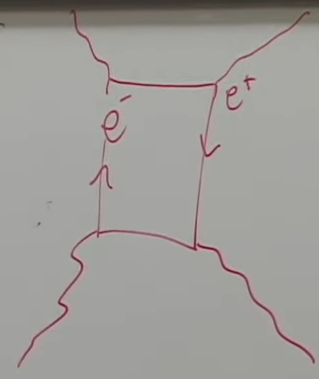
\includegraphics[width=0.8\textwidth]{2-6-photons}
 \end{figure}

\subsection{Spontaneous symmetry breaking}
 
\url{https://youtu.be/5rytN74EOi0?t=4824}

\section{Spontaneous symmetry breaking and Goldstone bosons}

TBP

\section{The Higgs field}

TBP

\section{The Higgs field and fermions}

TBP

\section{Renormalization and the running of coupling constants}

TBP

\begin{appendices}
	\section{Demystifying the Higgs Boson}
	\cite{susskind2010demystifing}
	TBP
\end{appendices}

\bibliographystyle{unsrt}
\addcontentsline{toc}{section}{Bibliography}
\raggedright
\bibliography{tm}


\end{document}
